\chapter{Glucose Microenvironment System}
\label{ch:glucose}

Understanding how tumors starve the immune system is central to designing effective therapies. This chapter introduces the glucose field that models this metabolic warfare --- and reveals a critical tipping point that determines whether the immune system wins or loses.

This chapter describes the glucose concentration field that overlays the discrete agent grid, modeling metabolic dynamics within the tumor microenvironment. The system captures diffusion, source injection from blood vessels, consumption by tumor and immune cells, and gradient-based chemotaxis for immune cell navigation.

%% ====================================================================
\section{Biological Motivation}
\label{sec:glucose-bio}

\begin{figure}[htbp]
\centering
\adjustbox{max width=0.85\textwidth, max height=0.7\textheight}{% Warburg Effect: Normal vs Cancer Cell Metabolism
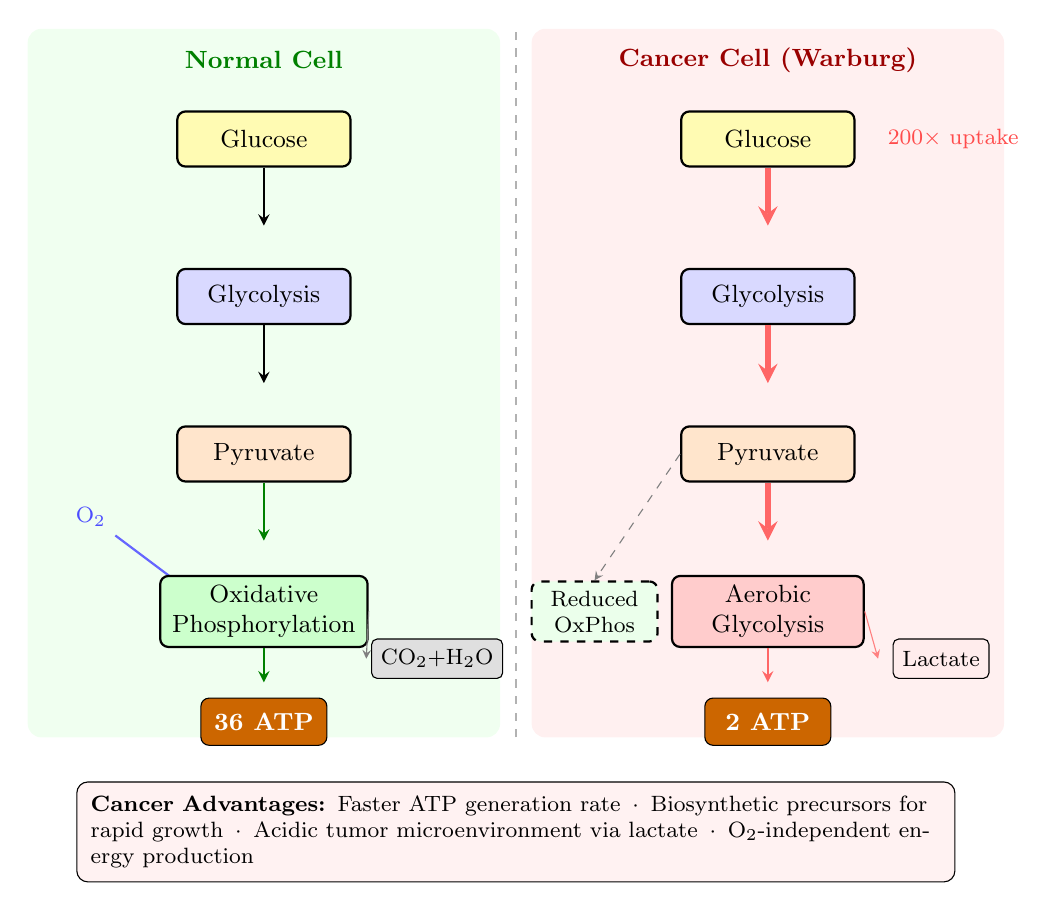
\begin{tikzpicture}[
  box/.style={draw, rounded corners=3pt, minimum width=2.2cm, minimum height=0.7cm,
              align=center, font=\small, thick},
  atp/.style={draw, rounded corners=3pt, font=\small\bfseries, text=white, fill=orange!80!black,
              minimum width=1.6cm, minimum height=0.6cm, align=center},
  byproduct/.style={draw, rounded corners=2pt, font=\footnotesize, fill=gray!25,
                    minimum height=0.5cm, align=center},
  arrow/.style={->, >=stealth, thick},
  fatarrow/.style={->, >=stealth, line width=2pt},
]

% Background panels
\fill[green!6, rounded corners=5pt] (-3.2, -0.4) rectangle (2.8, 8.6);
\fill[red!6, rounded corners=5pt] (3.2, -0.4) rectangle (9.2, 8.6);

% Panel headers
\node[font=\small\bfseries, green!50!black] at (-0.2, 8.2) {Normal Cell};
\node[font=\small\bfseries, red!60!black] at (6.2, 8.2) {Cancer Cell (Warburg)};

% Dividing line
\draw[dashed, gray!60, thick] (3.0, -0.4) -- (3.0, 8.6);

% === Normal Cell (left column, centered at x=0) ===
\node[box, fill=yellow!30] (gn) at (-0.2, 7.2) {Glucose};
\draw[arrow] (gn) -- ++(0, -1.1);

\node[box, fill=blue!15] (gly_n) at (-0.2, 5.2) {Glycolysis};
\draw[arrow] (gly_n) -- ++(0, -1.1);

\node[box, fill=orange!20] (pyr_n) at (-0.2, 3.2) {Pyruvate};
\draw[arrow, green!50!black] (pyr_n) -- ++(0, -1.1);

% O2 input
\node[font=\footnotesize, blue!70] (o2) at (-2.4, 2.4) {O$_2$};
\draw[arrow, blue!60] (o2) -- (-1.2, 1.5);

\node[box, fill=green!20, text width=2.4cm] (oxphos) at (-0.2, 1.2) {Oxidative\\Phosphorylation};
\draw[arrow, green!50!black] (oxphos) -- ++(0, -0.9);

\node[atp] (atp_n) at (-0.2, -0.2) {36 ATP};

\node[byproduct] at (2.0, 0.6) {CO$_2$+H$_2$O};
\draw[->, >=stealth, thin, gray] (oxphos.east) -- (1.1, 0.6);

% === Cancer Cell (right column, centered at x=6.2) ===
\node[box, fill=yellow!30] (gc) at (6.2, 7.2) {Glucose};
\node[font=\footnotesize, red!70, right] at (7.6, 7.2) {200$\times$ uptake};
\draw[fatarrow, red!60] (gc) -- ++(0, -1.1);

\node[box, fill=blue!15] (gly_c) at (6.2, 5.2) {Glycolysis};
\draw[fatarrow, red!60] (gly_c) -- ++(0, -1.1);

\node[box, fill=orange!20] (pyr_c) at (6.2, 3.2) {Pyruvate};
\draw[fatarrow, red!60] (pyr_c) -- ++(0, -1.1);

\node[box, fill=red!20, text width=2.2cm] (aero) at (6.2, 1.2) {Aerobic\\Glycolysis};
\draw[arrow, red!60] (aero) -- ++(0, -0.9);

\node[atp] (atp_c) at (6.2, -0.2) {2 ATP};

% Lactate
\node[byproduct, fill=pink!30] (lac) at (8.4, 0.6) {Lactate};
\draw[->, >=stealth, thin, red!50] (aero.east) -- (7.6, 0.6);

% Dashed branch to reduced OxPhos
\node[box, fill=green!8, font=\footnotesize, dashed, minimum width=1.6cm] (rox) at (4.0, 1.2) {\footnotesize Reduced\\OxPhos};
\draw[->, >=stealth, dashed, gray] (pyr_c.west) -- (rox.north);

% === Bottom advantages box (full width) ===
\node[draw, rounded corners=4pt, fill=red!5, text width=10.8cm, align=left, font=\footnotesize,
      inner sep=5pt] at (3.0, -1.6) {%
\textbf{Cancer Advantages:}\enspace
Faster ATP generation rate \,$\cdot$\,
Biosynthetic precursors for rapid growth \,$\cdot$\,
Acidic tumor microenvironment via lactate \,$\cdot$\,
O$_2$-independent energy production};

\end{tikzpicture}
}
\caption{The Warburg effect: metabolic competition in the tumor microenvironment}
\label{fig:warburg_effect}
\end{figure}

The metabolic landscape of the tumor microenvironment plays a decisive role in determining immune-tumor interactions. Otto Warburg observed that tumor cells preferentially metabolize glucose through aerobic glycolysis, resulting in dramatically elevated glucose uptake (up to 200-fold compared to normal tissue). This metabolic competition between tumor cells and infiltrating immune cells creates nutrient gradients that shape spatial organization, as regions surrounding tumor masses become nutrient-deprived. T cells and NK cells critically depend on glucose availability for cytotoxic activity — when glucose is scarce, T cell proliferation is impaired, IFN-$\gamma$ production decreases, and cytotoxic granule release is diminished. In the absence of direct cell-cell contact, immune cells can follow glucose concentration gradients as a proxy for proximity to functional vasculature and viable tissue, providing a chemotactic fallback behavior.

\begin{figure}[htbp]
\centering
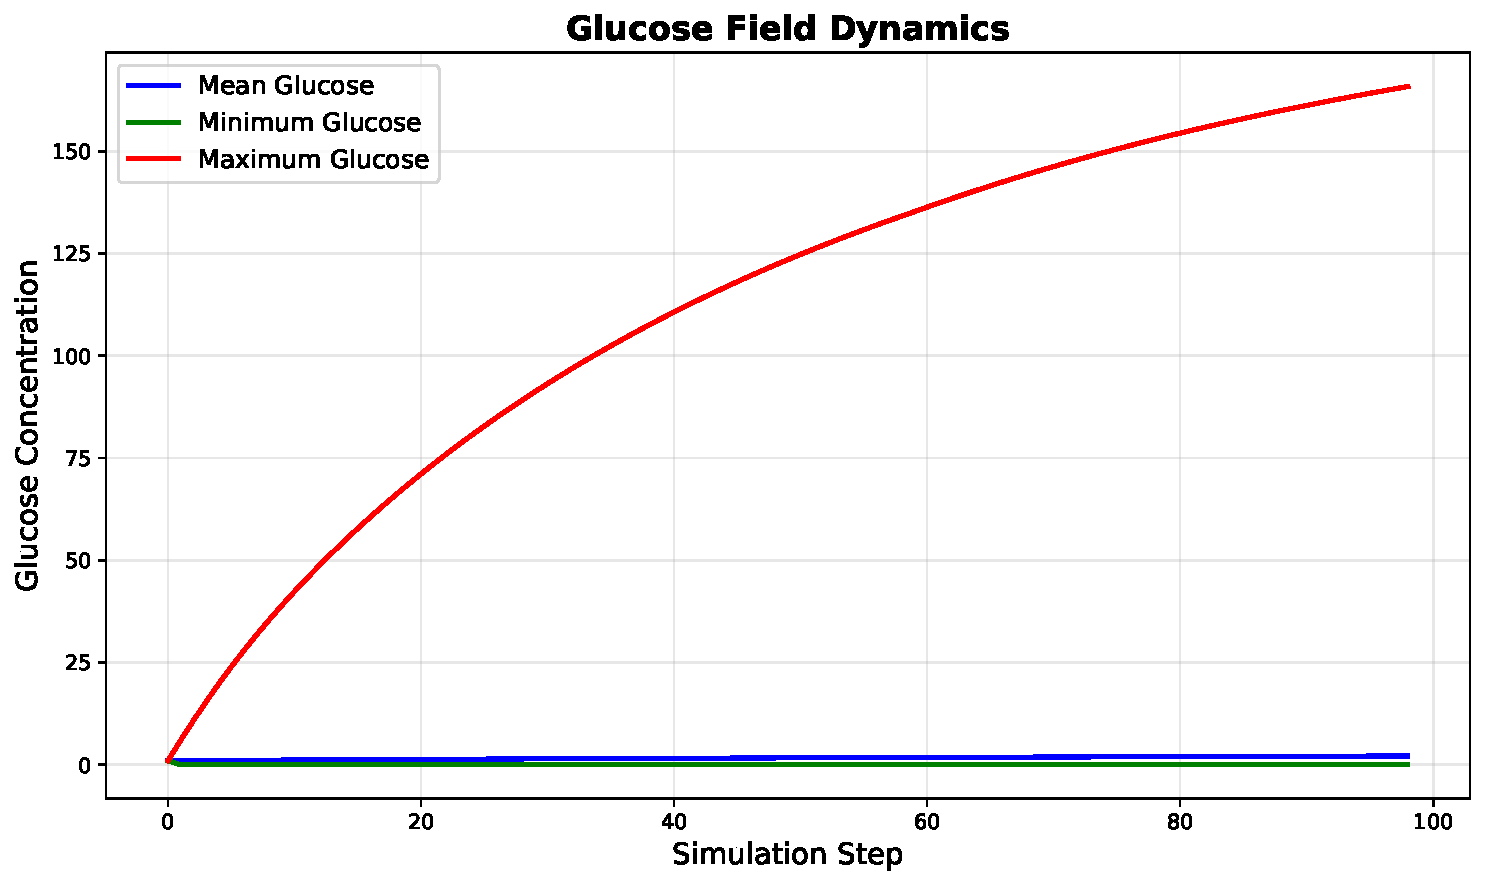
\includegraphics[width=0.85\textwidth]{figures/glucose_dynamics.pdf}
\caption{Glucose field dynamics over time showing the evolution of glucose concentration patterns in response to tumor growth and treatment. The spatial distribution reveals zones of depletion around tumor masses and gradients extending from blood vessel sources.}
\label{fig:glucose_dynamics}
\end{figure>

\begin{figure}[htbp]
\centering
\adjustbox{max width=0.85\textwidth, max height=0.7\textheight}{% Glucose System Block Diagram
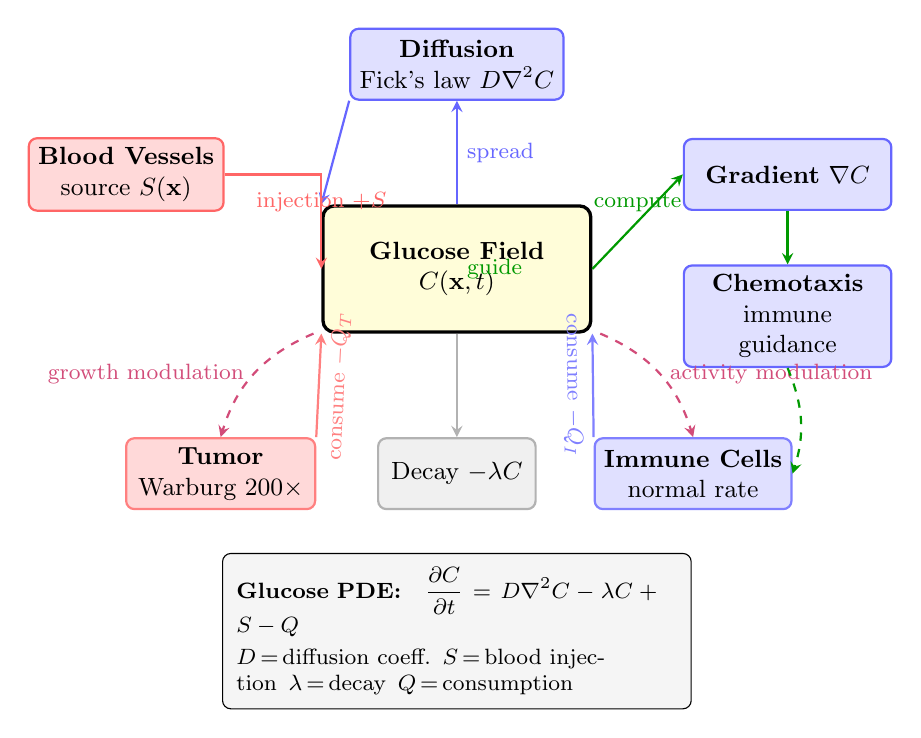
\begin{tikzpicture}[
  block/.style={draw, rounded corners=3pt, minimum width=2.4cm, minimum height=0.9cm,
                align=center, font=\small, thick},
  field/.style={draw, rounded corners=4pt, minimum width=3.4cm, minimum height=1.6cm,
                align=center, font=\small, thick, fill=yellow!15, line width=1.2pt},
  src/.style={block, fill=red!15, draw=red!60},
  proc/.style={block, fill=blue!12, draw=blue!60},
  cons/.style={block, fill=orange!15, draw=orange!60},
  arrow/.style={->, >=stealth, thick},
  dasharrow/.style={->, >=stealth, thick, dashed, purple!70},
]

% Central field
\node[field] (F) at (0, 0) {\textbf{Glucose Field}\\$C(\mathbf{x},t)$};

% Top: Diffusion
\node[proc] (diff) at (0, 2.6) {\textbf{Diffusion}\\Fick's law $D\nabla^2 C$};
\draw[arrow, blue!60] (F.north) -- (diff.south) node[midway, right, font=\footnotesize] {spread};
\draw[arrow, blue!60] (diff.south west) -- (F.north west);

% Left: Blood Vessels source
\node[src] (bv) at (-4.2, 1.2) {\textbf{Blood Vessels}\\source $S(\mathbf{x})$};
\draw[arrow, red!60] (bv.east) -- (F.west |- bv) -- (F.west)
  node[midway, above, font=\footnotesize] {injection $+S$};

% Right: Gradient & Chemotaxis
\node[proc, text width=2.4cm] (grad) at (4.2, 1.2) {\textbf{Gradient} $\nabla C$};
\node[proc, text width=2.4cm] (chem) at (4.2, -0.6) {\textbf{Chemotaxis}\\immune guidance};
\draw[arrow, green!60!black] (F.east) -- (grad.west) node[midway, above, font=\footnotesize] {compute};
\draw[arrow, green!60!black] (grad) -- (chem);

% Bottom-left: Tumor consumer
\node[cons, fill=red!15, draw=red!50] (tum) at (-3.0, -2.6) {\textbf{Tumor}\\Warburg 200$\times$};
\draw[arrow, red!50] (tum.north east) -- (F.south west)
  node[midway, below, sloped, font=\footnotesize] {consume $-Q_T$};

% Bottom-right: Immune consumer
\node[cons, fill=blue!12, draw=blue!50] (imm) at (3.0, -2.6) {\textbf{Immune Cells}\\normal rate};
\draw[arrow, blue!50] (imm.north west) -- (F.south east)
  node[midway, below, sloped, font=\footnotesize] {consume $-Q_I$};

% Below center: Decay
\node[proc, fill=gray!12, draw=gray!60, minimum width=2.0cm] (dec) at (0, -2.6) {Decay $-\lambda C$};
\draw[arrow, gray!60] (F.south) -- (dec.north);

% Dashed feedback arrows
\draw[dasharrow] (F.south west) ++(-0.1, 0) to[bend right=25]
  node[midway, left, font=\footnotesize, text=purple!70] {growth modulation} (tum.north);
\draw[dasharrow] (F.south east) ++(0.1, 0) to[bend left=25]
  node[midway, right, font=\footnotesize, text=purple!70] {activity modulation} (imm.north);

% Chemotaxis feedback
\draw[arrow, green!60!black, dashed] (chem.south) to[bend left=20] (imm.east)
  node[midway, right, font=\footnotesize] {guide};

% PDE equation box
\node[draw, rounded corners=3pt, fill=gray!8, inner sep=5pt, font=\footnotesize,
      text width=5.6cm, align=left] (pde) at (0, -4.6) {%
\textbf{Glucose PDE:}\quad
$\displaystyle\frac{\partial C}{\partial t} = D\nabla^2 C - \lambda C + S - Q$\\[2pt]
$D$\,=\,diffusion coeff.\enspace
$S$\,=\,blood injection\enspace
$\lambda$\,=\,decay\enspace
$Q$\,=\,consumption};

\end{tikzpicture}
}
\caption{Glucose system architecture showing the diffusion field, sources from blood vessels, and consumption by cellular agents.}
\label{fig:glucose_system}
\end{figure>

%% ====================================================================
\section{Mathematical Formulation}
\label{sec:glucose-math}

The glucose concentration field $C(\mathbf{x}, t)$ evolves according to a reaction--diffusion equation derived from Fick's second law:

\begin{equation}
\label{eq:glucose-pde}
\frac{\partial C}{\partial t} = D\,\nabla^2 C \;-\; \lambda\,C \;+\; S(\mathbf{x}) \;-\; Q(\mathbf{x}),
\end{equation}

\noindent where $C(\mathbf{x}, t)$ is the glucose concentration, $D$ is the diffusion coefficient (\texttt{w\_glucose\_diffusion}, default $0.1$), $\lambda$ is the natural decay rate (\texttt{w\_glucose\_decay}, default $0.01$), $S(\mathbf{x})$ is the source term (glucose injection from blood vessels), and $Q(\mathbf{x})$ is the consumption term (uptake by tumor and immune cells).

The continuous Laplacian $\nabla^2 C$ is discretized on a regular 3D Cartesian grid using the standard 6-connected stencil, implemented as a 3D convolution using \texttt{scipy.ndimage.convolve}. The diffusion equation is advanced using explicit Euler integration with stability condition $D < 1/6$. Neumann (zero-flux) boundary conditions are enforced, corresponding to no glucose flux through simulation domain walls.

\subsection{Source and Consumption Models}

Blood vessel agents inject glucose at their grid positions at rate $r_{\text{source}}$ (\texttt{w\_glucose\_source\_rate}, default 5.0) per step. Tumor cells consume glucose reflecting the Warburg effect at rate $r_{\text{tumor}}$ (\texttt{w\_glucose\_tumor\_consumption}, default 2.0), while immune cells consume at lower rate $r_{\text{immune}}$ (\texttt{w\_glucose\_immune\_consumption}, default 0.5).

Tumor cell proliferation probability is modulated by glucose availability: $f_{\text{glucose}} = \min(1.0, C(\mathbf{x}_t) \cdot w_{\text{growth\_sensitivity}})$, and immune cell kill rates are similarly scaled: $f_{\text{immune}} = \min(1.0, C(\mathbf{x}_i) \cdot w_{\text{immune\_sensitivity}})$. When glucose is abundant ($C \geq 1.0$), activities proceed at full rate; as glucose drops below 1.0, functions are proportionally suppressed.

%% ====================================================================
\section{Gradient and Chemotaxis}
\label{sec:glucose-chemotaxis}

The glucose gradient is computed using central finite differences, and for agent movement on the integer grid, the continuous gradient is converted to discrete step directions using the sign function. Immune cells that implement glucose chemotaxis (\texttt{CytotoxicTCell}, \texttt{MacrophageM1}, \texttt{DendriticCell}, \texttt{NaturalKiller}) employ a fallback strategy where they first attempt to move towards nearby tumor cells, and if no target is found, they move in the direction of increasing glucose concentration with probability $p_{\text{chemo}}$ (\texttt{w\_glucose\_chemotaxis\_strength}, default 0.3).

%% ====================================================================
\section{Implementation}
\label{sec:glucose-impl}

The glucose system is encapsulated in the \texttt{GlucoseField} class. The glucose field is stored as a 3D NumPy array with \texttt{float64} precision, initialized uniformly to 1.0. Each simulation step executes three phases:

\begin{enumerate}
    \item \textbf{Injection}: Blood vessels inject glucose at their positions
    \item \textbf{Diffusion}: Apply discrete Laplacian convolution and Euler integration  
    \item \textbf{Decay}: Multiply field by $(1 - \lambda)$
\end{enumerate}

Agent-level consumption occurs within each agent's \texttt{step()} method. The implementation uses vectorized NumPy operations for field updates while maintaining individual agent-level consumption behavior. The class exposes aggregate statistics (mean, total, min, max concentrations) for tracking metabolic dynamics over time.

\begin{figure}[htbp]
\centering
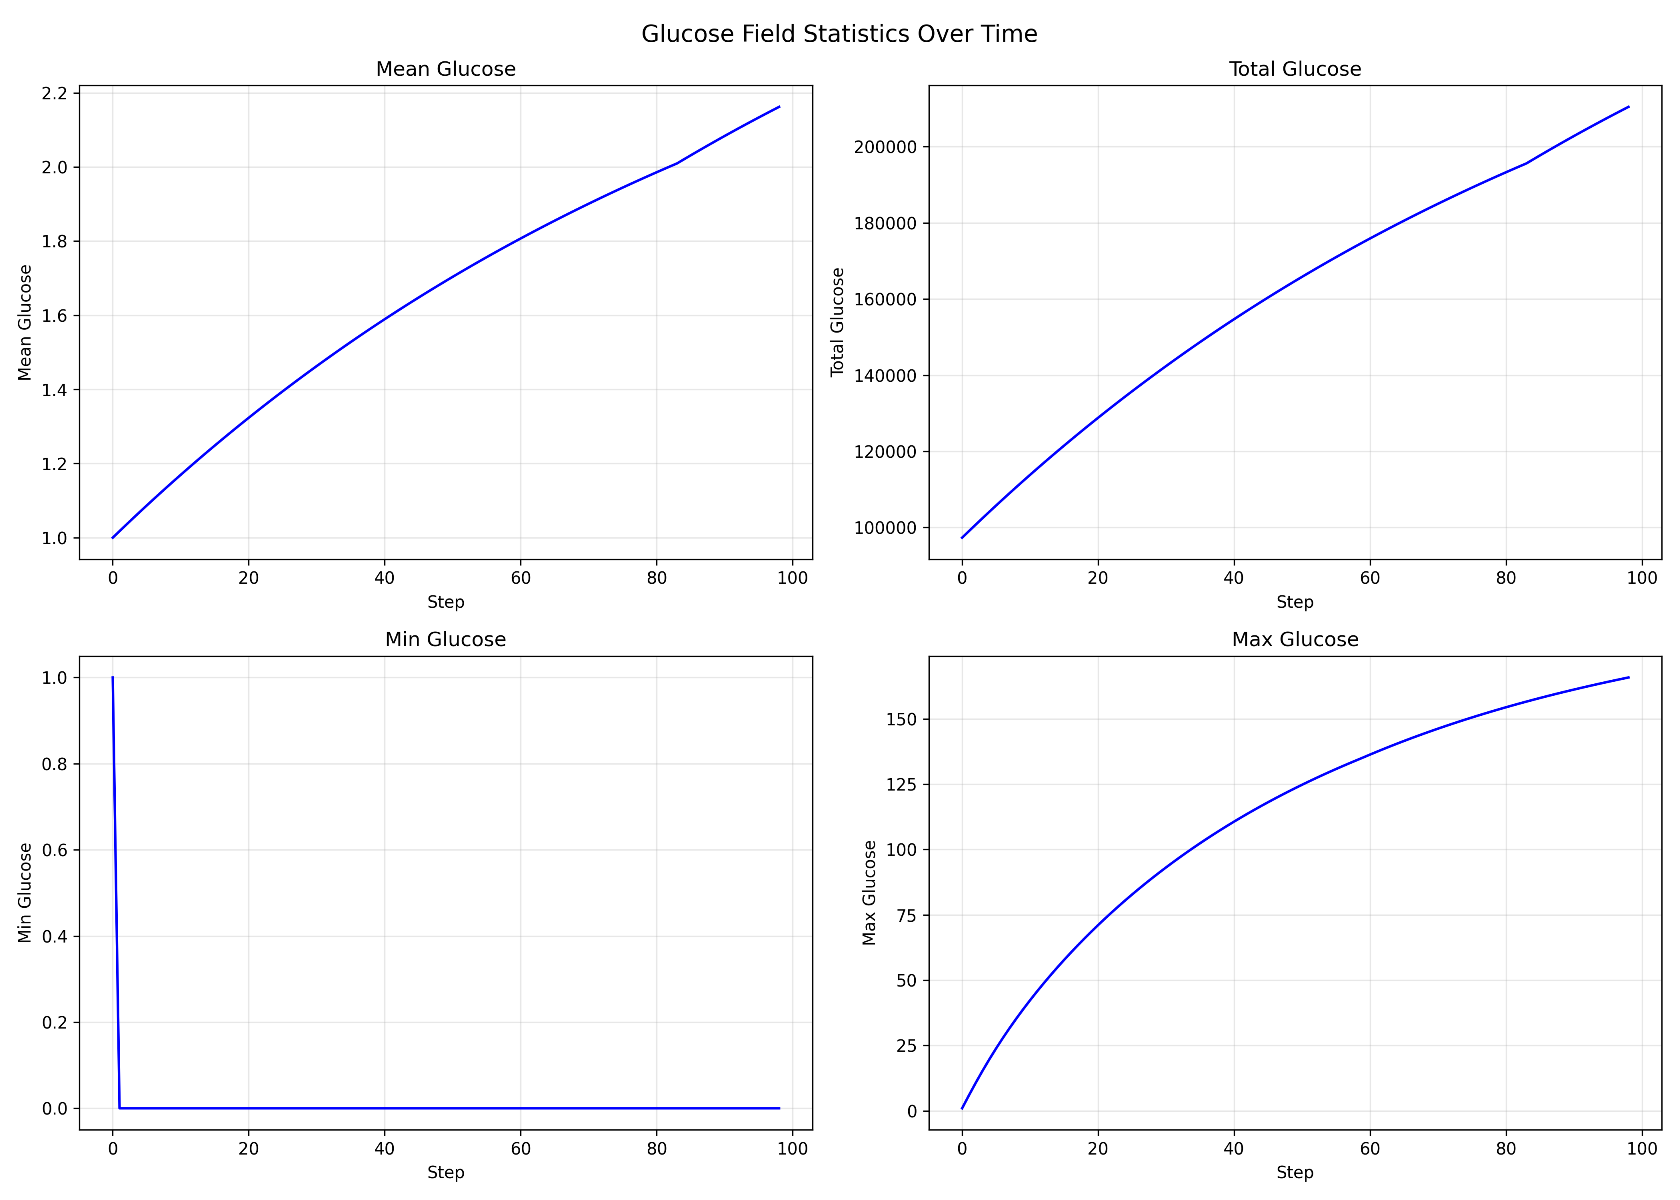
\includegraphics[width=0.85\textwidth]{figures/glucose_timeseries.pdf}
\caption{Glucose concentration time series showing the temporal evolution of mean, minimum, and maximum glucose levels throughout the simulation. The dynamics reflect the balance between blood vessel injection, cellular consumption, and spatial diffusion.}
\label{fig:glucose_timeseries}
\end{figure>

\begin{figure}[htbp]
\centering
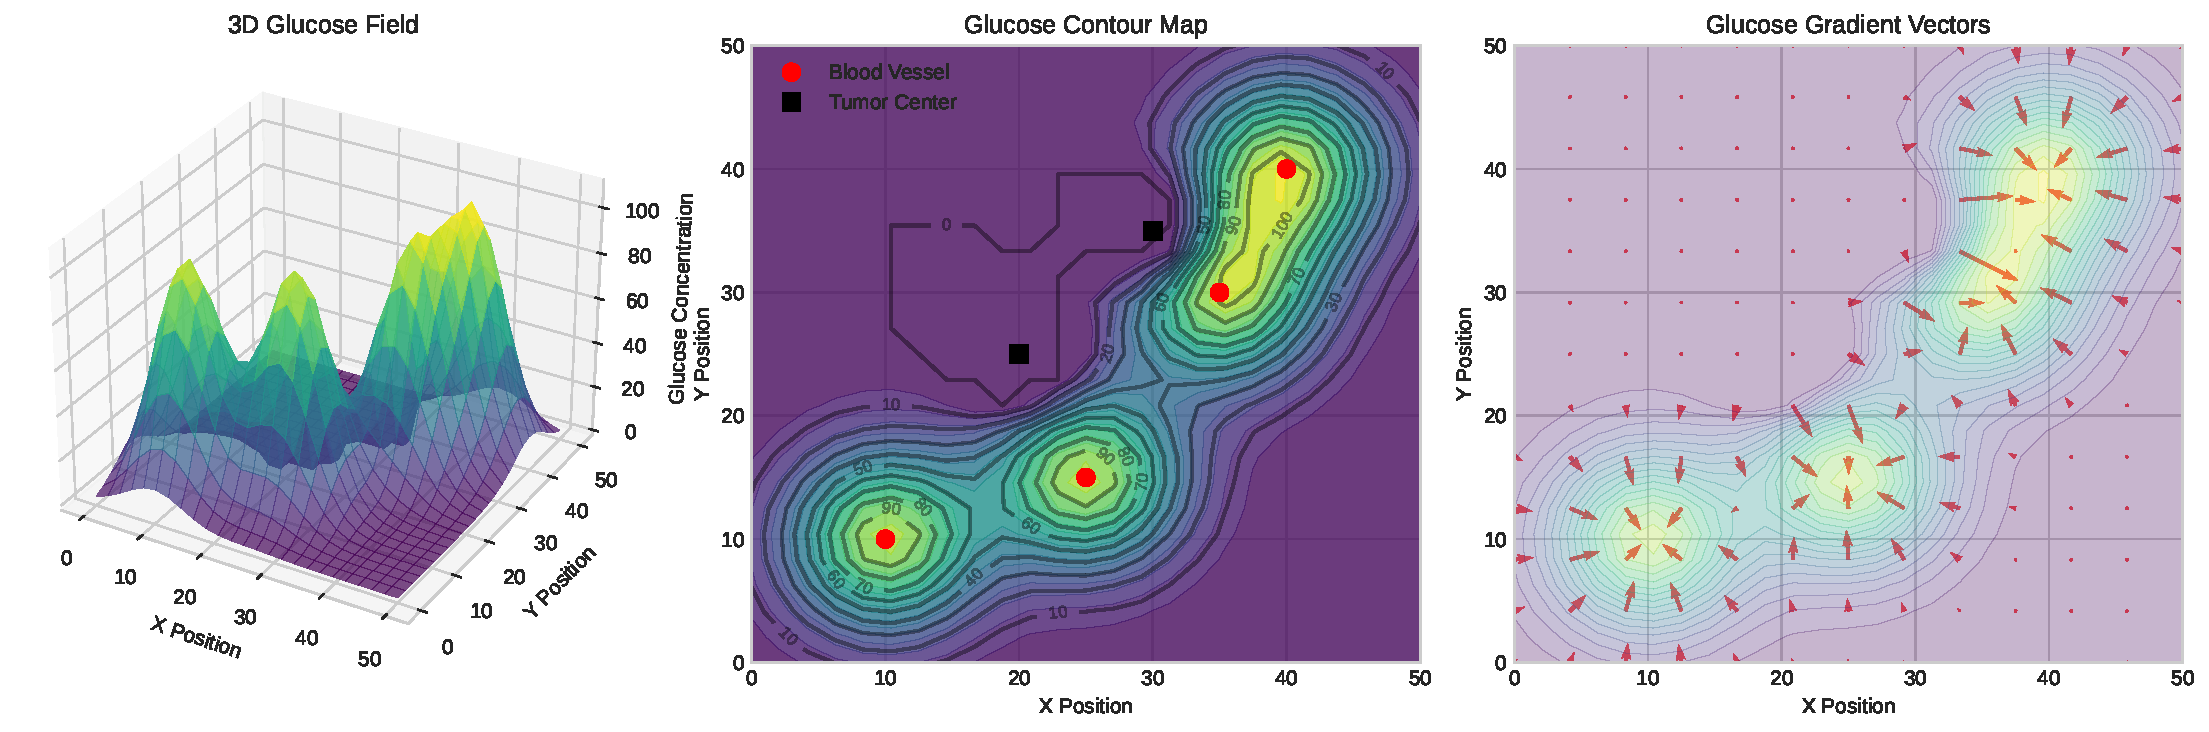
\includegraphics[width=0.85\textwidth]{figures/glucose_field_3d.pdf}
\caption{Three-dimensional visualization of the glucose concentration field showing spatial heterogeneity within the tumor microenvironment. High-concentration regions (yellow) correspond to blood vessel locations, while low-concentration zones (blue) indicate areas of intensive cellular consumption.}
\label{fig:glucose_field_3d}
\end{figure>

\begin{figure}[htbp]
\centering
\begin{tikzpicture}[
    node distance=2.5cm,
    source/.style={ellipse, draw, fill=blue!20, font=\small, minimum height=1.0cm, text width=1.8cm, text centered},
    process/.style={rectangle, draw, fill=green!15, font=\small, minimum height=1.0cm, text width=2.0cm, text centered, rounded corners=2pt},
    consumer/.style={rectangle, draw, fill=red!15, font=\small, minimum height=1.0cm, text width=1.8cm, text centered, rounded corners=2pt},
    effect/.style={rectangle, draw, fill=orange!15, font=\small, minimum height=1.0cm, text width=1.8cm, text centered, rounded corners=2pt},
    arrow/.style={->,>=stealth,thick},
    cycle_arrow/.style={->,>=stealth,thick,bend left=20}
]

% Central cycle nodes arranged in a circle
\node[source] (vessels) at (0,3) {Blood\\Vessels};
\node[process] (inject) at (2.5,2) {Glucose\\Injection};
\node[process] (diffusion) at (3,0) {Spatial\\Diffusion};
\node[consumer] (tumor) at (2,-2) {Tumor\\Consumption};
\node[consumer] (immune) at (-1,-2) {Immune\\Starvation};
\node[effect] (gradient) at (-3,0) {Concentration\\Gradient};
\node[effect] (chemotaxis) at (-2.5,2) {Immune\\Chemotaxis};

% Main cycle arrows
\draw[arrow] (vessels) -- (inject);
\draw[arrow] (inject) -- (diffusion);
\draw[arrow] (diffusion) -- (tumor);
\draw[arrow] (tumor) -- (immune);
\draw[arrow] (immune) -- (gradient);
\draw[arrow] (gradient) -- (chemotaxis);
\draw[arrow] (chemotaxis) -- (vessels);

% Additional effects
\node[font=\scriptsize, above=0.3cm of vessels] {Source};
\node[font=\scriptsize, right=0.3cm of diffusion] {Transport};
\node[font=\scriptsize, below=0.3cm of tumor] {Warburg Effect};
\node[font=\scriptsize, left=0.3cm of gradient] {Spatial Pattern};

% Central process annotation
\node[font=\small\bfseries] at (0.5,0) {Glucose Dynamics};

\end{tikzpicture}
\caption{Glucose System Cycle illustrating the circular flow of glucose dynamics in the tumor microenvironment.}
\label{fig:glucose_system_cycle}
\end{figure}